% !TEX options=--shell-escape
	\documentclass{article}
	\usepackage{amsmath,amssymb}
	\usepackage[inline]{enumitem}
	\usepackage{blindtext}
	\usepackage{booktabs}
	\usepackage{graphicx}
	\usepackage{xcolor}
	\usepackage[vmargin = 1.5in, top = 1in, bottom = 1.2in, letterpaper]{geometry}
	\usepackage{listings}
	\usepackage{courier}
	\usepackage{multicol}
	\usepackage{multirow}
	\usepackage{bm}
	\usepackage[title]{appendix}
	\usepackage[labelformat=simple]{subcaption}
	\renewcommand\thesubfigure{(\alph{subfigure})}
	\usepackage{minted}
	\usepackage{fvextra}
	\definecolor{bg}{rgb}{0.95,0.95,0.95}
	\newminted{r}{mathescape, breaklines, linenos = true, bgcolor = bg, fontsize = \footnotesize}
	\usemintedstyle{tango}
	% \lstset{
	% basicstyle = \small\tt,
	% keywordstyle = \tt\color{blue},
	% commentstyle = \it\color[cmyk]{1,0,1,0},
	% stringstyle = \tt\color[RGB]{128,0,0},
	% %frame = single,
	% backgroundcolor = \color[RGB]{245,245,244},
	% breaklines,
	% extendedchars = false,
	% xleftmargin = 2em,
	% xrightmargin = 2em,
	% aboveskip = 1em,
	% tabsize = 4,
	% showspaces = false
	% }
	\newcommand\inner[2]{\left\langle{#1},{#2}\right\rangle}
	\DeclareMathOperator{\Corr}{Corr}
	\DeclareMathOperator{\Cov}{Cov}
	\DeclareMathOperator{\Var}{Var}
	\DeclareMathOperator{\E}{E}
	\usepackage[round]{natbib}
	\usepackage{amsthm}

	\newtheorem{theorem}{Theorem}[section]
    \newtheorem{corollary}[theorem]{Corollary}
    \newtheorem{lemma}[theorem]{Lemma}

    \theoremstyle{definition}
    \newtheorem{definition}{Definition}[section]



	\begin{document}
	
	% \newfontfamily\courier{Courier New}

	
	\title{STAT 501 Project 2\\
	PCA for Discrete Distribution with Gaussian Copula}
	\author{Yifan Zhu}
	\maketitle
	\begin{abstract}
	In the report, we extend the semiparametric scale-invariant PCA method called copula PCA proposed by \cite{han2014high} to the case when our distribution is descrete. The senators' voting data set was used to apply this method. 
	\end{abstract}
	\section{Introduction}
	In this project, our goal is to reduce the dimension of catagorical data with PCA. However, we cannot perform PCA directly on the catagorical data, since the sample space only has finite points and we cannot find a proper set of basis (or principle components) for this space like what we did for continuous distribution. Hence we consider the catagorical data with descrete distribution are generated from some latent variables with continuous distribution. Then instead of performing PCA on the observed data, we perform PCA on the latent variables. We also want to transfrom or connect the latent variables to multivariable normal r.v.s. Since for dimension reduction, PCA is an optimal dimension reduction method for multivariate normal data. 
	\section{Method of copula PCA and extension to discrete case}
	\subsection{nonparanormal distribution}
	\begin{definition}[nonparanormal distribution, \cite{han2014high}] 
	Let $f^0 = \{f_j^0\}_{j=1}^d$ be a set of strictly increasing univariate functions. We say that a $d$ dimensional random vector $\bm X = (X_1, \ldots , X_d)^T$ follows a nonparanormal distribution $\mathrm{NPN}_d(\bm{\Sigma}_0, f^0)$, if
	\[f^0(\bm X) := (f_1^0 (X_1), \ldots, f_d^0(X_d))^T \sim \mathrm{N}_d(\bm 0, \bm{\Sigma}^0)\]
	where $\mathrm{diag}(\bm \Sigma^0) = \bm 1$.
	\end{definition}
	From the definition, the nonparanormal distribution must be a continuous distribution. And it is actually a special case of Gaussian copula family, when the distribution is continuous. 

	Suppose we have $\bm X \sim \mathrm{NPN}_d(\bm \Sigma^0, f^0)$, then the marginal cdfs are
	\[F_j(x_j) = P(X_j \leq x_j) = P(f_j^0(X_j) \leq f_j^0(x_j)) = \Phi(f_j^0(x_j))\]
	And the joint cdf is
	\begin{align*}
	F(x_1, x_2, \ldots, x_d) &= P(X_1 \leq x_1, \ldots, X_d \leq x_d) \\
	& = P(f_1^0(X_1) \leq f_1^0(x_1) ,\ldots, f_d^0(X_d) \leq f_d^0(x_d)) \\
	& = \Phi_{\bm \Sigma^0}(f_1^0(x_1), \ldots, f_d^0(x_d)))\\
	& = \Phi_{\bm \Sigma^0} (\Phi^{-1}(\Phi(f_1^0(x_1))), \ldots, \Phi^{-1}(\Phi(f_d^0(x_d))))\\
	& = \Phi_{\bm \Sigma^0}(\Phi^{-1}(F_1(x_1)), \ldots, \Phi^{-1}(F_d(x_d)))\\
	& = C_{\bm \Sigma^0}(F_1(x_1),\ldots, F_d(x_d))
		\end{align*}
		where $\Phi_{\bm \Sigma^{0}}$ is cdf of $\mathrm{N}_d(\bm 0, \bm \Sigma^{0})$ and $C_{\bm \Sigma^0}$ is a Gaussian copula with correlation matrix $\bm \Sigma^{0}$. So $\bm X \sin \mathrm{NPN}_d(\bm \Sigma^0, f^0)$ actually means $(F_1(X_1), \ldots, F_d(X_d))^T \sim C_{\bm \Sigma^0}$ or $(\Phi^{-1}(F_1(X_1)), \ldots, \Phi^{-1}(F_d(X_d)))^T \sim \mathrm{N}(\bm 0, \bm \Sigma^0)$. 

	\subsection{Estimation of $\bm \Sigma^0$}
	For nonparanormal distribution, we already know $F_j(x_j) = \Phi(f_j^0(x_j))$, then one natural way is to first estimate $f_j^0(x_j) = \Phi^{-1}(F_j(x_j))$, and then use the estimated $\hat{f}_j^0$ to transform the data to multivariate normal and estimate $\bm \Sigma^0$ as if we have data from a multivariate normal distribution. Suppose we have our data $\bm x_1, \ldots, \bm x_n$ from nonparanormal distribution, and $\bm x_i = (x_{i1}, \ldots, x_{id})^T$, then \cite{liu2012nonparanormal} gave an estimation of $f_j^0$ by
	\[\hat{f}_j^0 (t) = \Phi^{-1}\left(T_{\delta_n} [\hat{F}_j(t)]\right)\]
	where $T_{\delta_n}$ is a Winsorization (or truncation) operator defined as $T_{\delta_n}(x) = \delta_n I(x < \delta_n) + x I(\delta_n \leq x \leq 1 - \delta_n) + (1 - \delta_n) I(x > 1 - \delta_n)$ with $\delta_n = 1/(4n^{1/4} \sqrt{\pi \log n})$. And $\hat{F}_j(t) = \frac{1}{n+1} \sum_{i=1}^n I(x_{ij} \leq t)$ is the scaled empirical cdf of $X_j$. Then 
	\[\hat{\bm \Sigma}^0_{jk} = \frac{\frac{1}{n} \sum_{i=1}^n \hat{f}_j^0(x_{ij}) \hat{f}_{k}^0 (x_{ik})}{\sqrt{\frac{1}{n} \sum_{i=1}^n \left(\hat{f}_j^0 (x_{ij})\right)^2}\sqrt{\frac{1}{n} \sum_{i=1}^n \left(\hat{f}_k^0 (x_{ik})\right)^2}},\, \hat{\bm \Sigma}^0 = [\hat{\bm \Sigma}_{jk}^0]\]

	Another way to estimate $\bm \Sigma^0$ directly without estimating $f_j^0$ by \cite{liu2012nonparanormal} uses Spearman's $\rho$ and Kendall's $\tau$ statistics. Let $r_{ij}$ be the rank of $x_{ij}$ among $x_{1j}, \ldots, x_{nj}$ and $\bar{r}_j = \frac{1}{n} \sum_{i=1}^n r_{ij}$, then
	\begin{align*}
	&\hat{\rho}_{jk} = \frac{\sum_{i=1}^n (r_{ij} - \bar{r}_j)(r_{ik} - \bar{r}_k)}{\sqrt{\sum_{i=1}^n (r_{ij} - \bar{r}_j)^2 \cdot \sum_{i=1}^n (r_{ik} - \bar{r}_{k})}}\\
	&\hat{\tau}_{jk} = \frac{2}{n(n-1)} \sum_{1 \leq i < i' \leq n} \mathrm{sign}\left(x_{ij} - x_{i'j}\right)\left(x_{ik} - x_{i'k}\right)
	\end{align*}
	The population version of Spearman's $\rho$ and Kendall's $\tau$ are
	\[\rho_{jk} = \Corr(F_j(X_j), F_k(X_k)),\, \tau_{jk} = \Corr\left(\mathrm{sign}(X_j - \tilde{X}_j), \mathrm{sign}(X_k - \tilde{X}_k)\right)\]
	where $\tilde{X}_j$ and $\tilde{X}_k$ are two independent copies of $X_j$ and $X_k$.
	\begin{lemma}[\cite{liu2012nonparanormal}]\label{skeptic}
		Assuming $\bm X \sim \mathrm{NPN}(\bm \Sigma^0, f^0)$, we have
		\[\bm \Sigma_{jk}^0 = 2 \sin \left(\frac{\pi}{6} \rho_{jk}\right) = \sin \left(\frac{\pi}{2} \tau_{jk}\right)\]
	\end{lemma}
	By Lemma~\ref{skeptic}, we then estimate $\bm \Sigma^0$ by
	\[\hat{\bm \Sigma}^0_{jk} = 2 \sin \left(\frac{\pi}{6} \hat{\rho}_{jk}\right) = \sin\left(\frac{\pi}{2} \hat{\tau}_{jk}\right)\]

	For $\hat{\bm \Sigma}^0 = \left[2 \sin\left(\frac{\pi}{6} \hat{\rho}_{jk}\right)\right]$, \cite{han2014high} also showed when $\bm x_1, \bm x_2, \ldots, \bm x_n \overset{\mathrm{iid}}{\sim} \mathrm{NPN}_d(\bm \Sigma^0, f^0)$, for any $n > 21/{\log d} + 2$, 
	\[P\left(\|\hat{\bm \Sigma}^0 - \bm \Sigma^0\|_{\max} \leq 8 \pi \sqrt{\frac{\log d}{n}}\right) \geq 1 - \frac{2}{d^2}\]
	where $\|\bm M\|_{\max} = \max \{|\bm M_{ij}|\}$.

	Then we can use either estimation of $\bm \Sigma^0$ to perform our PCA. In \cite{han2014high} and \cite{han2013principal}, sparse assumption about the eigenvectors are imposed, and some theoratical properties were discussed about the sparse PCA solution. 


	\subsection{Generalized distributional transform and continuous latent variables}
	Now we want to extend the above method to catagorical case. The main idea is to define a latent continuous variable and apply the estimation of $\bm \Sigma^0$ with Spearman's $\rho$ and Kendall's $\tau$ (These two estimations both assume data are from continuous distribution). 
 	\begin{definition}[generalized distributional transformation, \cite{ruschendorf2013mathematical}, Chapter 1]
 	Let $Y$ be a real random variable with distribution function $F$ and let $V$ be a random variable independent of $Y$, such that $V \sim \mathrm{Uniform}(0,1)$. The generalized distributiona function is defined by
 	\[F(x, \lambda) = P(X < x) + \lambda P(Y = x)\]
 	and we call
 	\[U = F(Y, V)\]
 	the generalized distributional transform of $Y$.
	\end{definition}

	\begin{theorem}[\cite{ruschendorf2013mathematical}, Chapter 1]
	Let $U = F(Y, V)$ be the distributional transform of $Y$ as defined above, then
	\[U \sim \mathrm{Uniform}(0,1) \, \, \mathrm{and}\,\, Y = F^{-1}(U) \, \mathrm{a.s.} \] 
	where 
	\[F^{-1}(t) = \inf\{x \in \mathbb{R} : F(x) \geq t\}\]
	is the generalized inverse of $F$, or the quantile transform of $F$. 
	\end{theorem}

	Now suppose our $\bm X$ is from a discrete distribution of Gaussian copula family, then 
	\[F(x_1, \ldots, x_d) = C_{\bm \Sigma^0}(F_1(x_1), \ldots, F_d(x_d)),\]
	which means
	\[(U_1, \ldots, U_d)^T = (F_1(X_1, V_1), \ldots, F(X_d, V_d))^T \sim \mathrm{N}(\bm 0, \bm \Sigma^0)\]
	by Skalar's Theorem (see \cite{ruschendorf2013mathematical}).

	Thus we can consider $U_j = F_j(X_j, V_j),\, j = 1,\ldots,d$ to be our latent variables, where $F_j(x_j, 1) = P(X_j \leq x_j)$ is the marginal cdf of $\bm X$. And our data is generated by a quantile transformation of $U_j$, i.e. $X_j = F^{-1}_j (U_j)$ 

	To transform the catagorical data to the latent continuous one, we will use the empirical cdf and empirical pmf. Suppose for $X_j$ there are $m$ possible values which are $c_1 < c_2, \ldots, c_m$, then the empirical pmf is
	\[\hat{P}_j(c_l) = \frac{1}{n} \sum_{i=1}^n I(x_{ij} = c_l)\]
	and the empirical cdf is
	\[\hat{F}_j(t) = \sum_{i=1}^n I(x_{ij} \leq t)\]
	and 
	\[\hat{F}_j(c_l) = \sum_{k=1}^l \hat{P}_j(c_k)\]

	Then our transformation would be
	\[\hat{F}_j(c_l, V) = \hat{F}_j(c_{l-1}) + \hat{P}_j(c_l) V\]
	when $l = 1$, we denote $\hat{F}_j(c_0) = 0$.

	And the quantile transform would be
	\[\hat{F}_j^{-1} (u) = \sum_{k=1}^m c_k I(\hat{F}_j(c_{k-1}) < u \leq \hat{F}_j(c_k) )\]

	We perform the copula PCA with $\bm \Sigma^0$ estimated by Spearman's $\rho$ or Kendall's $\tau$ from the data we obtained with generalized distributional transformation. Then we can do dimension reduction for $(\Phi^{-1}(U_1), \ldots, \Phi^{-1}(U_d))^T$. We can also transform the data projected to a lower dimension back to the catagorical data and see the difference. 

	Also, we need to note that the estimated $\hat{\bm \Sigma^0}$ using this method might not be a correlation matrix (might not be positive and with 1's in the diagnal). Thus in practice we find the nearest correlation matrix of $\hat{\bm \Sigma}^0$ and use this correlation matrix to perform our PCA. Method used here is by \cite{higham2002computing} to find the nearest correlation matrix in terms of $\infty$ norm.

	\section{Senators' voting data set}
	We use senators' voting data to try this method. In this data set, there are 100 observations, each observation has 542 components. Possibles values are $-1, 0 ,1$. We first transform the data to continuous one with empirical marginal distribution and then calculate the estimation of $\bm \Sigma^0$. We can also test the multivariate normality, since a basic assumpution we made is that the data is from Gaussian copula family.

	We test the multivariate normality of the marginal transformed data by projecting the data to one dimension of some arbitrary directions, e.g. 10000 differeny directions. The p-value is \textbf{0.03988561}, which means our assumption that the data are from a Gaussian copula family might not hold. But we will still continue in spite of this.

	We used both Spearman's $\rho$ and Kendall's $\tau$ estimations. For Spearman's $\rho$, the first 38 and 58 PCs can account for 80\% and 90\% of the total variance . And for Kendall's $\tau$, the first 39 PCs and 61 PCs can account for 80\% and 90\% of the total variance. The cumulative proportion of total variance against number of PCs is shown in Figure~\ref{cpvar}.

	\begin{figure}[!htb]
	    \centering
		\begin{subfigure}[b]{0.45\textwidth}
		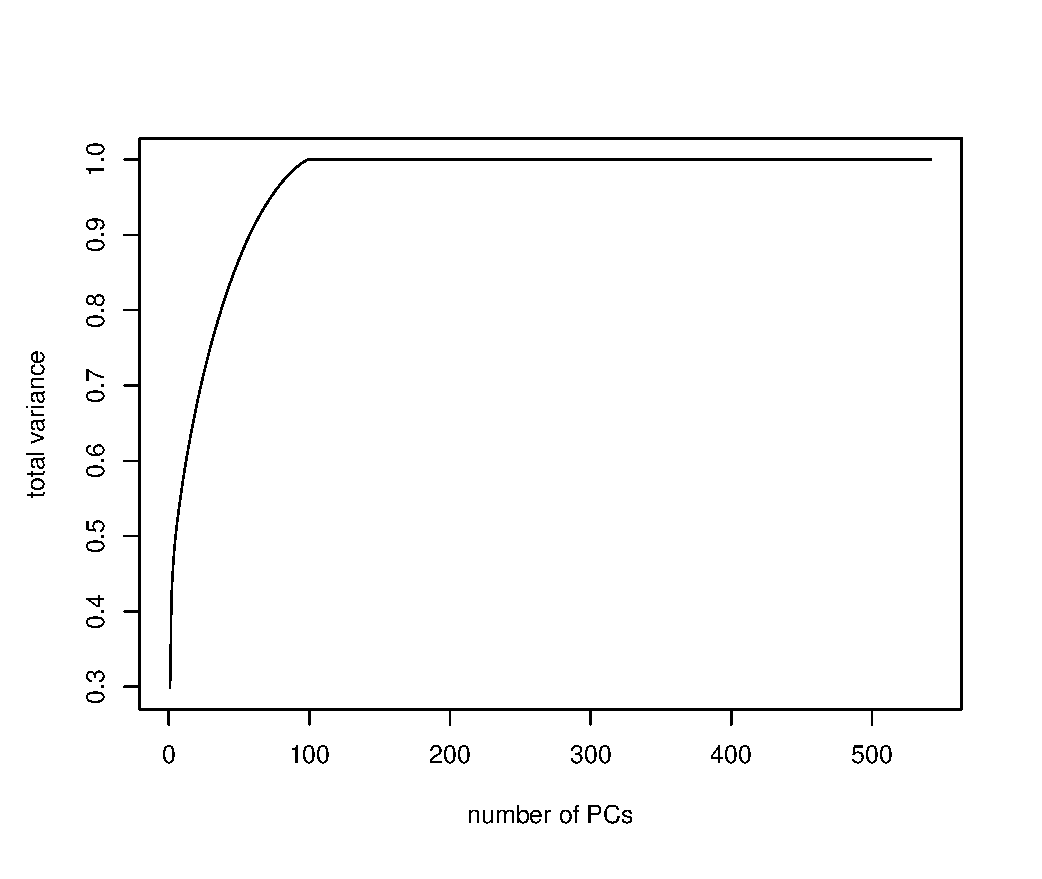
\includegraphics[width = \textwidth]{rho.eps}
		\caption{by estimation with Spearman's $\rho$}
		\end{subfigure}%
		\begin{subfigure}[b]{0.45\textwidth}
		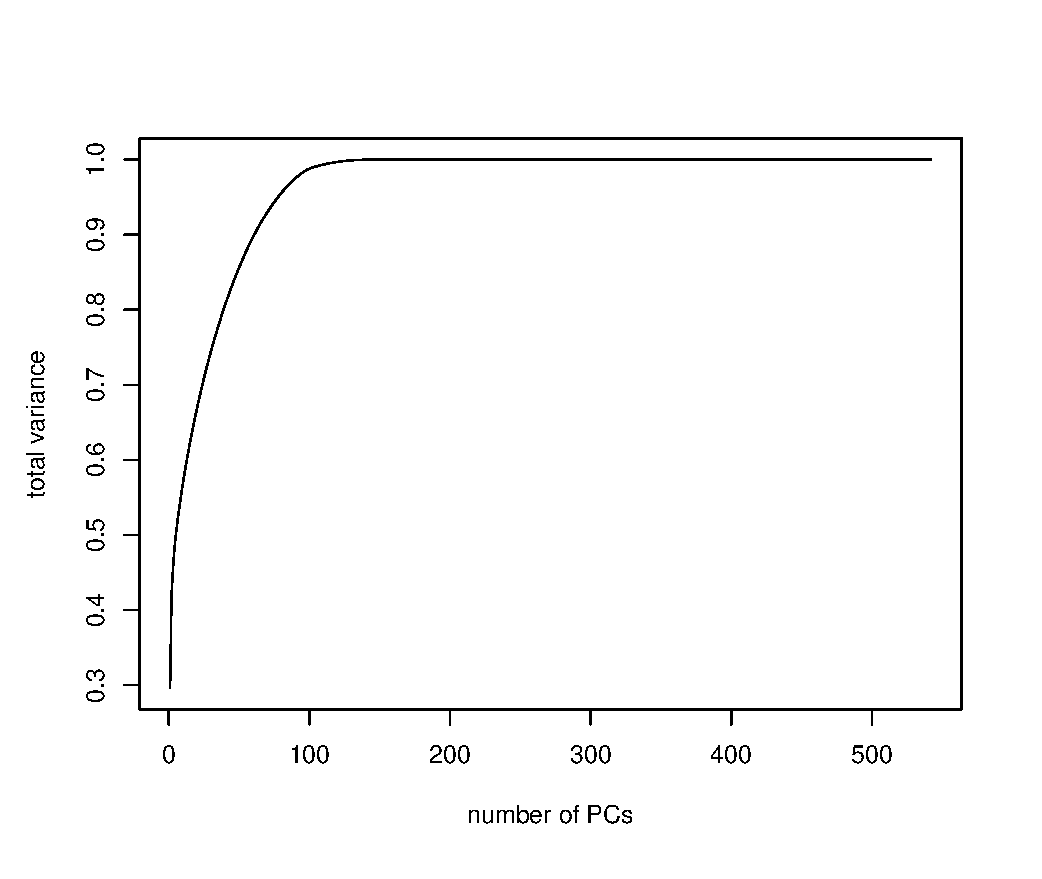
\includegraphics[width = \textwidth]{tau.eps}
		\caption{by estimation with Kendall's $\tau$}
		\end{subfigure}
		\caption{Cumulative proportion of variance against number of PCs with two kinds of estimations of correlation matrix}
		\label{cpvar}
	\end{figure}
	 Then we reconstruct the senators' voting data by these few PCs (number of PCs accounting for 80\% and 90\% of variance with estimation from Spearman's $\rho$ and Kendall's $\tau$) with the help of quantile transformation, and compare how much of our catagorical data matches with the original one. The percent of matched data is shown in Table~\ref{matching}. We can see we can reconstruct the data pretty well although our assumption is not reallt met here.

	\begin{table}[!htb]
		 	\caption{Percent of matching data between dimension reduced and original}
		 	\label{matching}
		 	\centering
		 	\begin{tabular}{ccc}
		 	\toprule
		 	& Spearman's $\rho$ & Kendall's $\tau$\\
		 	\midrule
		 	80\% & 0.9196863 & 0.9167159\\
		 	90\% & 0.9295387 & 0.9244834\\
		 	\bottomrule
		 	\end{tabular}
		 \end{table}

	\section{Discussion}
	We can see this method is pretty simple and performs well in the senators' voting data set. Although the assumption is not really met we still get good result: the dimension is reduced a lot and not a lot of information is lost. One reason might be our estimation is based one the rank information of data, and that provided some robustness when deviating from the assumption. We could invetigate about this in the future if possible.






    \bibliographystyle{plainnat}
	\bibliography{./project2.bib}
\newpage
\appendix
	\begin{appendices}
	\section{R codes}
	\begin{rcode}
library(readxl)
senators<-read_xls("senate_voting_data.xls")

#b) Plot Andrews' curves

senators.names<-names(senators)[-c(1,2)]
rev.party.state.names<-lapply(X=strsplit(gsub(pattern="[.]",replacement="",x=senators.names),split=" "),FUN = rev)

senators.party <- lapply(X = rev.party.state.names, FUN = function(x)(unlist(x)[1]))
senators.party <- unlist(senators.party)

senators.last.names <- lapply(X = rev.party.state.names, FUN = function(x)(unlist(x)[4]))
senators.last.names <- unlist(senators.last.names)


#Create new data.frame for plotting
senators_new <- as.data.frame(t(senators[,-c(1,2)]))

colnames(senators_new) <- NULL
rownames(senators_new) <- NULL

senators_new <- data.frame(senators_new, party = senators.party)


# Use the codes from Canvas
source("ggandrews.R")

# Display the Andrews' curves
ggandrews(senators_new, type = 2, clr = 543, linecol = c("blue", "green", "red"), return_value = FALSE)


epmf <- function(x){
  n <- length(x)
  return(c(sum(x==-1), sum(x==0), sum(x==1))/n)
}

ecdf <- function(epmf){
  return(c(0, epmf[1], epmf[1]+epmf[2], 1))
}

senator_epmf <- sapply(senators_new[,-ncol(senators_new)], epmf)
senator_ecdf <- apply(senator_epmf, MARGIN = 2, ecdf)

library(plyr)

gdtrans <- function(i){
  u1 <- mapvalues(senators_new[,i], from = c(-1,0,1), to = senator_epmf[,i])
  u2 <- mapvalues(senators_new[,i], from = c(-1,0,1), to = senator_ecdf[1:3,i])
  return(u2 + u1*runif(n = length(u1)))
}

inv_gdtrans <- function(u, i){
  -1* (senator_ecdf[1,i] < u[,i] & senator_ecdf[2,i] >= u[,i]) + 1* (senator_ecdf[3,i] < u[,i] & senator_ecdf[4,i] >= u[,i])
}

source("testnormality.R")



senators_c <- sapply(1:542, gdtrans)

senators_normal <- qnorm(senators_c, mean = 0, sd = 1)

testnormality(senators_normal)

library(energy)
mvnorm.etest(x = senators_normal, R = 1000)

library(MASS)
library(Matrix)

# rho based estimation
spearmanrho <- cor(senators_c, method = "spearman")
sigmahat_rho <- 2*sin(pi/6*spearmanrho)
sigmahat_rho <- nearPD(sigmahat_rho, corr = T)
decomp_rho <- eigen(sigmahat_rho$mat, symmetric = T)

s <- decomp_rho$values

pvar<-s/sum(s)

#  cumulative proportion of total variance explained 
#  by each component

cpvar <- cumsum(s)/sum(s)
plot(x = 1:length(cpvar), y = cpvar, 'n', xlab = 'number of PCs', ylab = 'total variance')
lines(x = 1:length(cpvar), y = cpvar)

npc80 <- min(which(cpvar > 0.8))
npc90 <- min(which(cpvar > 0.9))

senators_normal_80 <- senators_normal%*%decomp_rho$vectors[,1:npc80]%*%t(decomp_rho$vectors[,1:npc80])

senators_u_80 <- pnorm(senators_normal_80, mean = 0, sd = 1)

senators_80 <- sapply(1:542, inv_gdtrans, u = senators_u_80)

sum(senators_80==senators_new[,-ncol(senators_new)])/(542*100)


senators_normal_90 <- senators_normal%*%decomp_rho$vectors[,1:npc90]%*%t(decomp_rho$vectors[,1:npc90])

senators_u_90 <- pnorm(senators_normal_90, mean = 0, sd = 1)

senators_90 <- sapply(1:542, inv_gdtrans, u = senators_u_90)

sum(senators_90==senators_new[,-ncol(senators_new)])/(542*100)

# tau based estimation
kendalltau <- cor(senators_c, method = "kendall")
sigmahat_tau <- sin(pi/2*kendalltau)
sigmahat_tau <- nearPD(sigmahat_tau, corr = T)
decomp_tau <- eigen(sigmahat_tau$mat, symmetric = T)

s <- decomp_tau$values

pvar<-s/sum(s)

#  cumulative proportion of total variance explained 
#  by each component

cpvar <- cumsum(s)/sum(s)
plot(x = 1:length(cpvar), y = cpvar, 'n', xlab = 'number of PCs', ylab = 'total variance')
lines(x = 1:length(cpvar), y = cpvar)
npc80 <- min(which(cpvar > 0.8))
npc90 <- min(which(cpvar > 0.9))

senators_normal_80 <- senators_normal%*%decomp_tau$vectors[,1:npc80]%*%t(decomp_tau$vectors[,1:npc80])

senators_u_80 <- pnorm(senators_normal_80, mean = 0, sd = 1)

senators_80 <- sapply(1:542, inv_gdtrans, u = senators_u_80)

sum(senators_80==senators_new[,-ncol(senators_new)])/(542*100)


senators_normal_90 <- senators_normal%*%decomp_tau$vectors[,1:npc90]%*%t(decomp_tau$vectors[,1:npc90])

senators_u_90 <- pnorm(senators_normal_90, mean = 0, sd = 1)

senators_90 <- sapply(1:542, inv_gdtrans, u = senators_u_90)

sum(senators_90==senators_new[,-ncol(senators_new)])/(542*100)

	\end{rcode}
	\end{appendices}








	
	
	
	\end{document}